% MSDM5054 Project 1 report. NeurIPS-like layout that compiles offline.
% To use the official style on Overleaf: replace the geometry/times lines by
%   \usepackage[preprint]{neurips_2024}   (after uploading neurips_2024.sty)
\documentclass[10pt]{article}
\usepackage[letterpaper,textwidth=5.5in,textheight=9in,top=1in]{geometry}
\usepackage{times}
\usepackage{graphicx,booktabs,amsmath,hyperref,xcolor,caption,subcaption,natbib}
\hypersetup{colorlinks=true,linkcolor=blue,urlcolor=blue,citecolor=blue}
\newcommand{\todo}[1]{\textcolor{red}{[TODO: #1]}}
\newcommand{\fig}[2]{\IfFileExists{#1}{\includegraphics[width=#2]{#1}}{\fbox{\parbox{#2}{\centering\vspace{2em}\texttt{\detokenize{#1}} not yet generated\vspace{2em}}}}}
\newcommand{\NTrain}{307,511}
\newcommand{\DefaultRate}{8.07\%}
\newcommand{\NFeatAll}{339}
\newcommand{\NFeatApp}{131}
\newcommand{\AucLogit}{0.7505}
\newcommand{\AucLgbApp}{0.7686}
\newcommand{\AucLgbAll}{0.7926}
\newcommand{\KagglePublic}{0.79713}
\newcommand{\KagglePrivate}{0.79295}
\newcommand{\AucIndOnly}{0.5849}
\newcommand{\ThinShare}{14.3\%}
\newcommand{\RobSeeds}{TBD}
\newcommand{\RobAucAll}{TBD}
\newcommand{\RobAucAllSd}{TBD}
\newcommand{\RobGainThin}{TBD}
\newcommand{\RobGainThick}{TBD}
\newcommand{\RobGainDiff}{TBD}
\newcommand{\RobGainDiffSd}{TBD}
\newcommand{\RobHolds}{TBD}


\title{Beyond the Leaderboard: Informative Missingness and Thin-File Borrowers in Home Credit Default Prediction}
\author{ZHANG Qi (21358199) \quad DU Yunhe (21419400) \quad TANG Yunshu (21275921) \quad WEI Fanjing (21354557)\\ Kaggle team: \texttt{msdm5054-zhang-du-tang-wei}\\ MSDM5054 Statistical Machine Learning, Project 1}
\date{}

\begin{document}
\setlength{\abovecaptionskip}{4pt}\setlength{\belowcaptionskip}{4pt}
\setlength{\textfloatsep}{10pt}\setlength{\intextsep}{8pt}
\maketitle

\begin{abstract}
We study default prediction on the Home Credit Default Risk data (\NTrain{} loans, default rate \DefaultRate{}), asking not only how accurately default can be predicted but for whom and why. A gradient-boosted model on the application table and six auxiliary tables reaches a 5-fold out-of-fold (OOF) AUC of \AucLgbAll{} (Kaggle private score \KagglePrivate{}), compared with \AucLogit{} for a regularized logistic regression. We then pose two scientific questions. First, is missingness informative? A model that sees \emph{only which fields are missing} attains AUC \AucIndOnly{}, well above chance, yet making that information explicit changes predictive performance by less than 0.002 AUC --- the missingness signal is almost entirely redundant given the observed covariates. Second, does the model serve ``thin-file'' applicants, the \ThinShare{} with no credit-bureau history, as well as others? They default more often (10.1\% versus 7.7\%) and are ranked less accurately (AUC 0.779 versus 0.794), but alternative data helps them substantially more (AUC gain $+0.032$ versus $+0.023$, non-overlapping bootstrap intervals): it narrows the gap without closing it. We close by discussing selection bias in the observed loan population, which limits what any model trained on these data can claim.
\end{abstract}

\section{Introduction}
Credit scoring for applicants with limited credit history is both a statistical and a social problem. Home Credit, a lender focused on the underbanked, supplements application data with alternative sources such as previous applications, point-of-sale and installment payment histories. Most public solutions to the associated Kaggle competition focus on maximizing AUC through feature engineering and ensembling. We treat predictive performance as the starting point and ask three questions:
\begin{itemize}\itemsep0pt
\item \textbf{RQ1 (Missingness).} Many application fields are missing for large fractions of applicants. Is the fact that a field is missing itself predictive of default, and how should missing values therefore be handled?
\item \textbf{RQ2 (Thin-file applicants).} \ThinShare{} of applicants have no record in the credit-bureau data. Are discrimination and calibration worse for them, and does alternative data narrow the gap?
\item \textbf{RQ3 (Drivers).} Which features drive predictions, and are their effects directionally plausible?
\end{itemize}
Our contributions are (i) a reproducible, leakage-free pipeline aggregating all seven tables; (ii) a systematic comparison of missing-data strategies; (iii) a subgroup analysis of discrimination and calibration with bootstrap intervals; and (iv) a discussion of how sample selection limits the conclusions.

\section{Data}
The training set contains \NTrain{} applications with a binary default label; the test set contains 48,744 unlabeled applications. Six auxiliary tables link to applications by client ID: bureau records of credits at other institutions and their monthly balances, previous Home Credit applications, and monthly histories of point-of-sale/cash loans, installment payments and credit cards. Two anomalies are handled explicitly: \texttt{DAYS\_EMPLOYED} equals 365,243 for about 18\% of applicants (a placeholder, predominantly for pensioners), which we set to missing while keeping a binary flag; and \texttt{CODE\_GENDER} has a few \texttt{XNA} values, set to missing. \todo{one sentence on the extent of missingness, e.g. how many columns exceed 50\% missing}

\section{Methods}
\textbf{Features.} From the application table we construct domain ratios (credit/income, annuity/income, annuity/credit as a proxy for repayment rate, goods price/credit, employment length/age, income per family member), summaries of the three external scores, and the count of missing fields. Each auxiliary table is aggregated to the client level (mean, maximum, minimum or sum of numeric fields; record counts; shares of categorical levels; and, for installments, days past due, days before due, payment shortfall and share of late payments). The final design has \NFeatAll{} features (\NFeatApp{} from the application table).

\textbf{Models.} (a) $L_2$-regularized logistic regression ($C=0.05$) with median imputation plus missingness indicators, one-hot encoding and standardization; (b) LightGBM \citep{ke2017lightgbm} with learning rate 0.03, 32 leaves, at least 100 samples per leaf, row subsampling 0.8, column subsampling 0.5, $L_2$ penalty 5 and early stopping (200 rounds). All models use 5-fold stratified cross-validation; we report OOF AUC and average fold models for test predictions.

\textbf{RQ1.} For every field with 1--99\% missing we compare the default rate when missing versus observed. We fit a logistic model on binary missingness indicators alone, and compare four strategies on application features: median imputation and median imputation plus indicators (logistic), and LightGBM with native missing-value handling versus after median imputation.

\textbf{RQ2.} Thin-file applicants are those with no bureau record. Per group we compute OOF AUC and Brier score for the application-only and all-tables LightGBM models, the AUC gain from auxiliary tables with a 95\% bootstrap interval (300 resamples), and decile calibration curves.

\textbf{RQ3.} Exact TreeSHAP contributions \citep{lundberg2020local} via LightGBM's \texttt{pred\_contrib} on a fixed sample of 50,000 applications, ranked by mean absolute contribution.

\section{Results}
\begin{table}[h]\centering\small
\caption{Predictive performance (5-fold OOF AUC) and Kaggle late-submission scores.}\label{tab:main}
\begin{tabular}{llccc}
\toprule
Model & Features & OOF AUC & Kaggle public & Kaggle private\\
\midrule
Logistic regression (L2) & application & 0.7505 & -- & --\\
LightGBM & application & 0.7686 & -- & --\\
LightGBM & all tables & 0.7926 & 0.79713 & 0.79295\\
\bottomrule
\end{tabular}

\end{table}

\textbf{Performance.} Two increments are visible in Table~\ref{tab:main}. Replacing logistic regression by gradient boosting on the same application features adds $0.018$ AUC ($0.7505 \to 0.7686$), indicating that non-linearities and interactions among application fields carry real signal that a linear log-odds model cannot express. Adding the six auxiliary tables adds a further $0.024$ AUC ($0.7686 \to 0.7926$), a larger gain than the change of model class: what the applicant did in the past with other lenders and with Home Credit matters more than a richer functional form on the application form alone.

\begin{table}[h]\centering\small
\caption{RQ1: missing-data strategies on application features (OOF AUC).}\label{tab:missing}
\begin{tabular}{lc}
\toprule
Strategy (application features) & OOF AUC\\
\midrule
Missingness indicators only (logistic) & 0.5849\\
Logistic, median imputation & 0.7493\\
Logistic, median imputation + indicators & 0.7505\\
LightGBM, native NaN handling & 0.7686\\
LightGBM, median-imputed & 0.7684\\
\bottomrule
\end{tabular}

\end{table}

\begin{figure}[h]\centering
\fig{fig_rq1_missing.png}{0.82\textwidth}
\caption{RQ1: default rate when a field is missing versus observed, for the fields with the largest difference.}\label{fig:missing}
\end{figure}

\textbf{RQ1: missingness is informative but redundant.} Missingness is clearly associated with the outcome: a logistic model using \emph{only} 61 binary missingness indicators, with no observed values at all, reaches AUC \AucIndOnly{} (Table~\ref{tab:missing}); Figure~\ref{fig:missing} shows the fields whose presence or absence separates defaulters most strongly.

How it is handled, however, barely matters. Adding missingness indicators to the logistic model moves AUC from $0.7493$ to $0.7505$ ($+0.0012$), and LightGBM with native missing-value handling ($0.7686$) is indistinguishable from LightGBM trained after median imputation ($0.7684$; the difference, $-0.0002$, is far smaller than the spread across folds). We read this as a redundancy result rather than a negative one: missingness does carry information about default, but essentially all of it is recoverable from the observed covariates, so an explicit encoding adds nothing. This is a useful caution against the common practice of adding missingness indicators reflexively and reporting the resulting model as evidence that ``missingness is informative''. These patterns are consistent with outcome-related (informative) missingness. The observed data cannot, however, distinguish missing-at-random from missing-not-at-random, because the mechanism depends on unobserved values \citep{little2019statistical}.

\begin{table}[h]\centering\small
\caption{RQ2: discrimination and calibration by group (OOF). Gain = AUC(all tables) $-$ AUC(application only).}\label{tab:thin}
\resizebox{\textwidth}{!}{\begin{tabular}{lrcccccc}
\toprule
Group & $n$ & Default & AUC (app) & AUC (all) & Gain [95\% CI] & Brier (all)\\
\midrule
all & 307,511 & 8.07\% & 0.7686 & 0.7926 & +0.0239 [+0.0222, +0.0256] & 0.0655\\
thin-file (no bureau) & 44,020 & 10.12\% & 0.7475 & 0.7794 & +0.0319 [+0.0275, +0.0364] & 0.0803\\
with bureau history & 263,491 & 7.73\% & 0.7708 & 0.7936 & +0.0227 [+0.0211, +0.0242] & 0.0630\\
\bottomrule
\end{tabular}
}
\end{table}

\begin{figure}[h]\centering
\begin{subfigure}{0.48\textwidth}\centering\fig{fig_rq2_calibration.png}{\linewidth}\caption{Calibration by group.}\end{subfigure}
\begin{subfigure}{0.48\textwidth}\centering\fig{fig_rq3_top20.png}{\linewidth}\caption{Top-20 features by mean $|$SHAP$|$.}\end{subfigure}
\caption{RQ2 calibration and RQ3 feature contributions.}\label{fig:rq23}
\end{figure}

\textbf{RQ2: thin-file applicants.} Thin-file applicants are 14.3\% of the sample and default markedly more often (10.1\% versus 7.7\%). The model ranks them less accurately: with the full feature set, AUC is $0.7794$ for thin-file applicants against $0.7936$ for those with bureau history. The auxiliary tables, however, help the thin-file group more --- a gain of $+0.0319$ $[0.0275, 0.0364]$ against $+0.0227$ $[0.0211, 0.0242]$ for the rest, with non-overlapping bootstrap intervals. Alternative data therefore does what it is advertised to do, narrowing the performance gap for applicants without traditional credit records, but it does not close it: even after adding every auxiliary table, discrimination for thin-file applicants remains below the application-only performance achieved for applicants with bureau history. Brier scores are not comparable across groups here because the base rates differ, so calibration is read from Figure~\ref{fig:rq23}(a) instead.

\textbf{RQ3: drivers.} The mean of the three external credit scores dominates by a wide margin (mean $|$contribution$|$ $0.32$ on the log-odds scale, three times the next feature), followed by demographic and loan-structure variables (\texttt{CODE\_GENDER}, \texttt{AMT\_ANNUITY}, \texttt{PAYMENT\_RATE}, \texttt{GOODS\_CREDIT}) and by aggregates of the auxiliary tables (\texttt{BURO\_\allowbreak DEBT\_\allowbreak CREDIT\_\allowbreak MAX}, the timing of previous instalment schedules, total amounts paid, and the share of late instalments). The directions are economically sensible: higher external scores and lower debt-to-credit ratios lower predicted risk, while a higher annuity-to-credit ratio --- a shorter, heavier repayment schedule --- raises it. Two observations connect back to RQ1. First, the individual external scores still appear below \texttt{EXT\_MEAN}, i.e.\ the model mostly uses their average, which is defined even when one of them is missing. Second, no missingness-derived feature (\texttt{N\_MISSING\_APP}, \texttt{DAYS\_EMPLOYED\_ANOM}) enters the top twenty, which is exactly what the redundancy result in the RQ1 results above predicts; the one apparent exception, \texttt{OWN\_CAR\_AGE} (66\% missing), contributes through its observed values rather than through an indicator.

\textbf{SHAP profiles: thin-file vs.\ with bureau.} Repeating the RQ3 decomposition separately for the two RQ2 groups (Figure~\ref{fig:shapgroups}) shows \emph{where} the thin-file discrimination deficit comes from. For applicants with bureau history, the single most relied-upon bureau feature, \texttt{BURO\_\allowbreak DEBT\_\allowbreak CREDIT\_\allowbreak MAX} (mean $|$SHAP$|$ $0.118$), is close to unusable for thin-file applicants ($0.044$, a gap of $-0.074$), and reliance on \texttt{EXT\_SOURCE\_3} drops by a similar margin ($0.098 \to 0.041$), largely because that score is itself missing for a large share of thin-file applicants. The model compensates by leaning harder on what it can still observe: the averaged external score \texttt{EXT\_MEAN} ($0.314 \to 0.375$, $+0.061$), \texttt{EXT\_SOURCE\_2} ($+0.018$), and --- notably --- the Home-credit-internal alternative-data aggregates \texttt{INS\_\allowbreak AMT\_\allowbreak PAYMENT\_\allowbreak SUM} and \texttt{INS\_\allowbreak LATE\_\allowbreak MEAN} ($+0.014$ each), which thin-file applicants \emph{can} have because the thin-file definition only excludes Credit-Bureau records, not previous Home Credit activity. This pattern is consistent with the RQ2 gain for thin-file applicants being driven mainly by internal behavioural data rather than by bureau data --- mean $|$SHAP$|$ measures reliance, not a decomposition of the AUC gain, so we read it as corroboration rather than proof. It sharpens the RQ2 interpretation: what helps financially excluded applicants is not more credit-bureau information (which does not exist for them) but alternative in-house payment histories.

\begin{figure}[h]\centering
\fig{fig_shap_group_comparison.png}{0.86\textwidth}
\caption{Group-wise TreeSHAP profiles (fold-0 model, 50{,}000-row sample; 7{,}214 thin-file rows). (a) Mean $|$SHAP$|$ per feature for each group; (b) the difference thin-file $-$ with-bureau (red: the model relies on the feature more for thin-file applicants).}\label{fig:shapgroups}
\end{figure}

The dependence profiles (Figure~\ref{fig:dependence}) confirm that the dominant effects are monotone and economically sensible, with two caveats worth flagging. \texttt{EXT\_MEAN} ($\rho=-0.99$) is almost perfectly linear in the log-odds --- the model treats the external score average as a near-deterministic risk scale. \texttt{BURO\_\allowbreak DEBT\_\allowbreak CREDIT\_\allowbreak MAX} ($\rho=+0.73$) is flat and mildly risk-reducing below a ratio of $1$, then jumps sharply once recorded debt exceeds the credited amount --- a plausible distress signal, though the small cluster of values far above $1$ (clipped in the figure) most likely reflects reporting glitches rather than genuine behaviour, and the model may be reading noise there. The applicant's gender enters as an almost binary split (male $+$0.1--0.3, female $-0.1$--$-0.15$ log-odds): it is the second most important feature overall, which is statistically unsurprising but raises a fairness concern for deployment, since gender is a protected attribute in most lending regulation; we report it as a property of the data-generating process rather than endorse its use. Finally, \texttt{AMT\_ANNUITY} ($\rho=+0.94$) and \texttt{GOODS\_CREDIT} ($\rho=-0.91$) act as smooth, monotone loan-structure controls; neither shows a sign reversal, so no interaction pathology is suspected at the top of the ranking.

\begin{figure}[h]\centering
\fig{fig_shap_dependence_top5.png}{0.88\textwidth}
\caption{SHAP dependence for the five most important features (colour: applicant group; grey diamonds: feature value missing; continuous features clipped to their 0.5--99.5th percentile for display; $\rho$ = Spearman correlation of feature vs.\ SHAP among observed values).}\label{fig:dependence}
\end{figure}

\textbf{Alternative-data source ablation.}

The full LightGBM model achieves an OOF AUC of 0.7926 using all seven
tables. To determine whether the predictive value of alternative data is
uniformly distributed across sources, we performed a controlled
leave-one-source-out ablation. All experiments used the same feature
engineering pipeline, LightGBM hyperparameters, random seed, and five-fold
stratified cross-validation. We removed one auxiliary source at a time from
the full 339-feature design and measured the resulting change in OOF ROC-AUC.

\begin{table}[t]
\centering
\small
\caption{Leave-one-source-out ablation of alternative financial data sources.}
\label{tab:ablation}
\begin{tabular}{lrr}
\toprule
Removed source & OOF AUC & $\Delta$ AUC \\
\midrule
None (full model) & 0.792586 & 0.000000 \\
Bureau & 0.786724 & +0.005862 \\
Previous applications & 0.790105 & +0.002481 \\
POS/CASH & 0.792853 & -0.000267 \\
Installments & 0.789636 & +0.002950 \\
Credit cards & 0.791226 & +0.001361 \\
\bottomrule
\end{tabular}
\end{table}

Bureau features provide the largest marginal contribution: removing them
reduces OOF AUC by 0.005862. Installment-payment and previous-application
histories provide smaller but still noticeable contributions, while
credit-card history has a relatively limited marginal effect. In contrast,
removing POS/CASH produces a negligible increase in AUC of 0.000267,
suggesting little additional discrimination once the other historical
sources are available. This should not be interpreted as evidence that
POS/CASH is harmful, since the experiment uses a single fixed
cross-validation configuration and does not quantify uncertainty around
this small difference.

Overall, the results indicate that the predictive value of alternative data
is heterogeneous: different historical sources do not contribute equally
to overall default discrimination.

\begin{figure}[t]
\centering
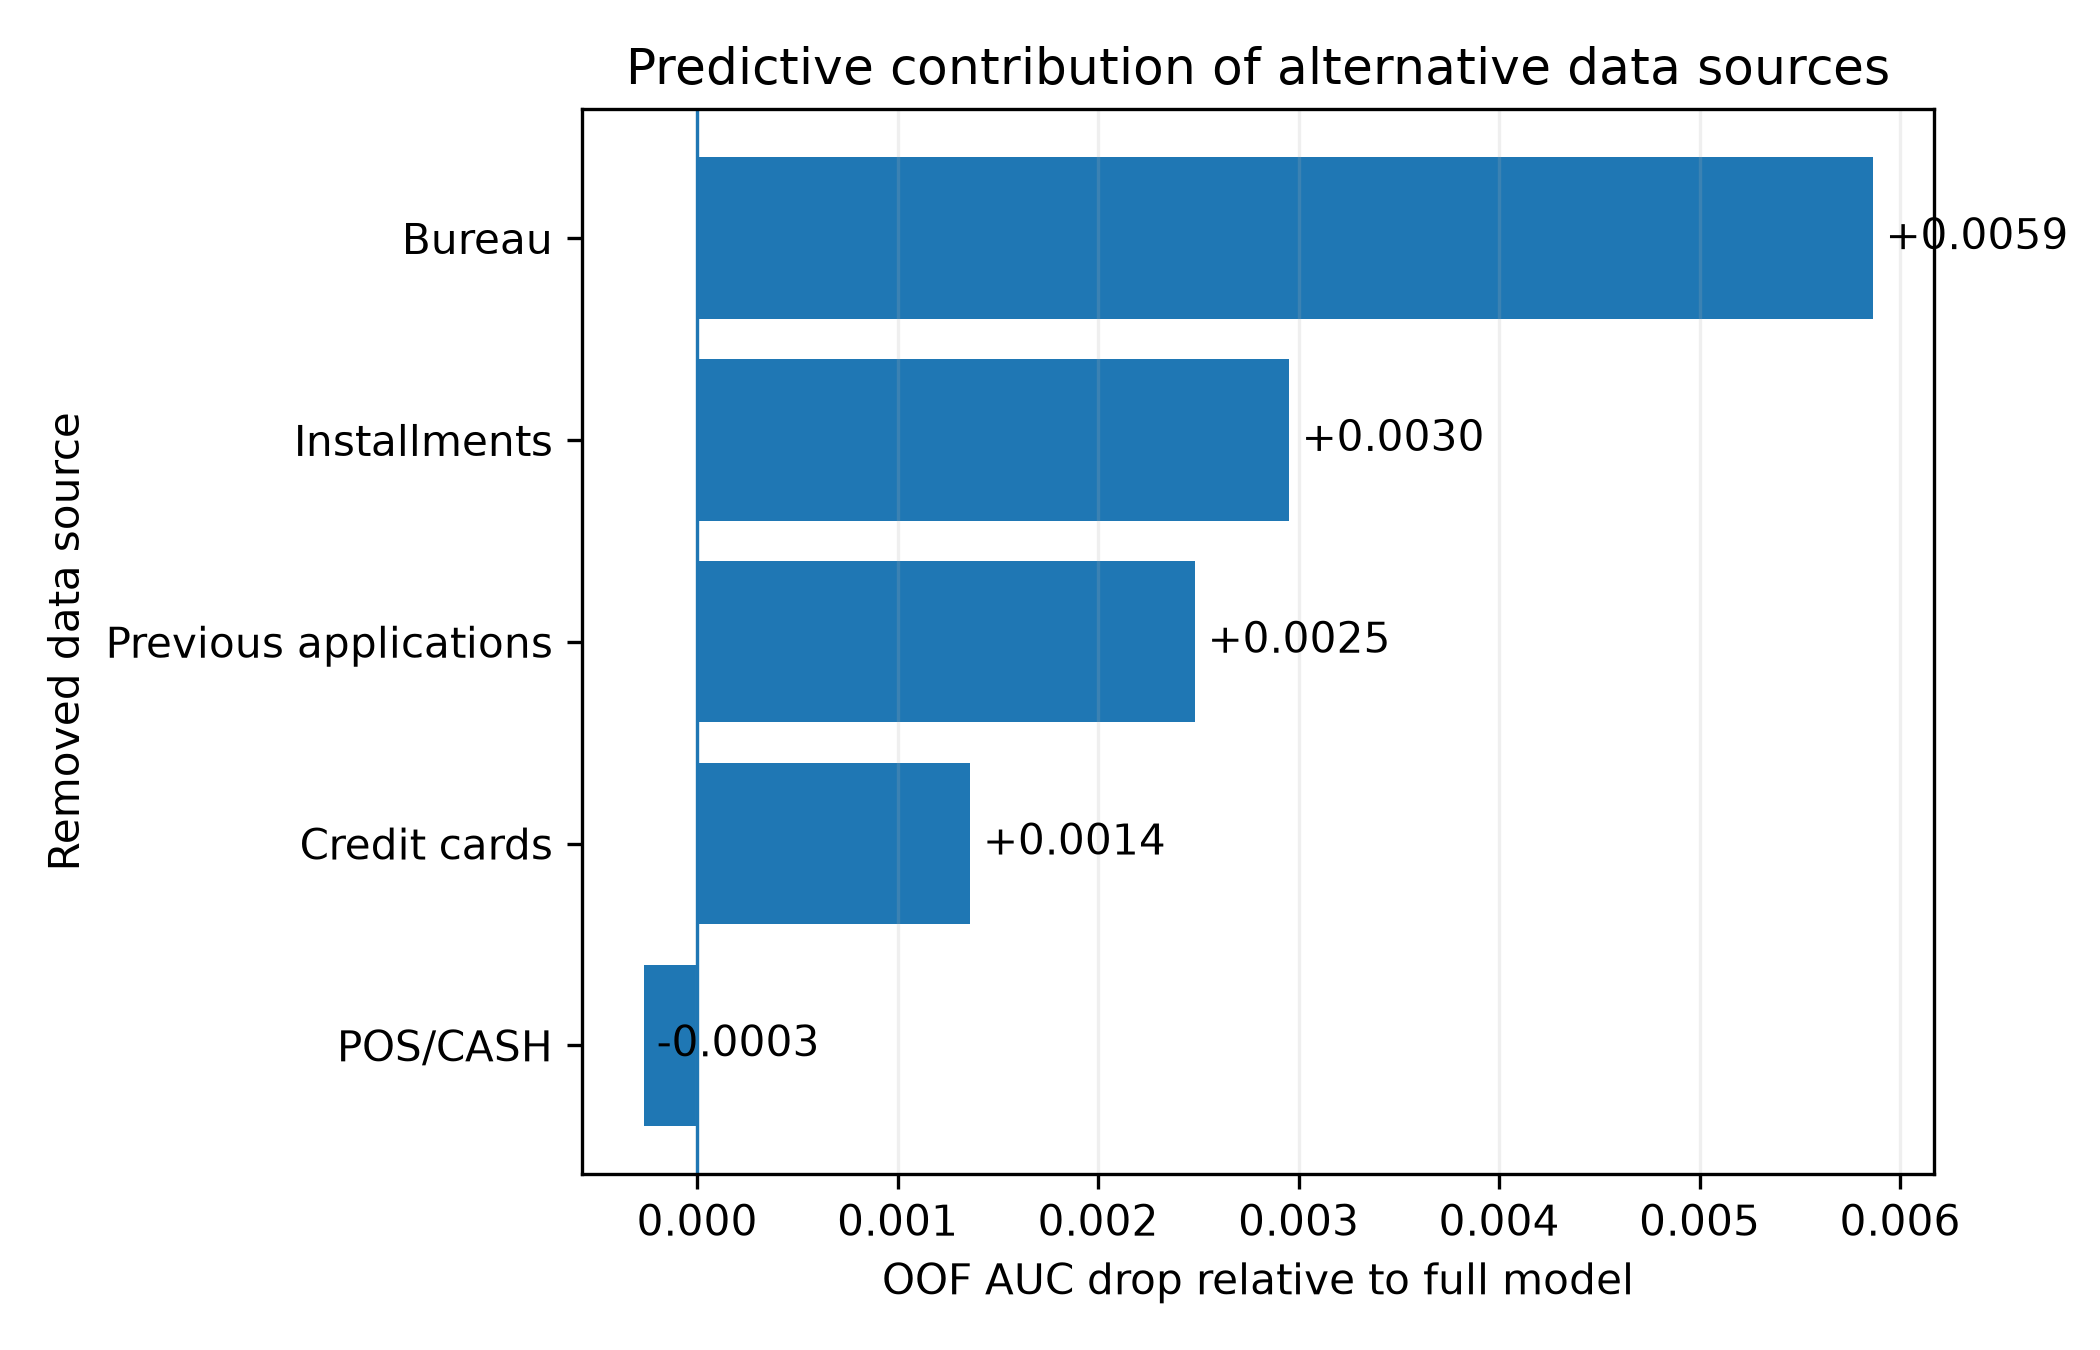
\includegraphics[width=0.85\linewidth]{fig_ablation_auc.png}
\caption{Decrease in OOF ROC-AUC after removing each alternative financial
data source from the full model. Larger values indicate greater marginal
predictive contribution.}
\label{fig:ablation}
\end{figure}

Read together with the group-wise SHAP profiles, the ablation also explains the thin-file deficit: the single most valuable auxiliary source for the population as a whole is exactly the one that does not exist for thin-file applicants, so the sources that remain available to them are individually weaker.

\textbf{Robustness.} All results above come from a single seed (42). To check that our conclusions are not seed-specific, we repeated the two LightGBM configurations and the RQ1 logistic comparison under five random seeds (Table~\ref{tab:robustness}).\footnote{The robustness runs were executed on a LightGBM build that rejects pandas categorical columns, so categorical features were passed as integer codes; the seed-42 column therefore differs from Table~\ref{tab:main} by at most $0.0014$ AUC. All other results, including the ablation, use the native categorical handling of Table~\ref{tab:main}.} The all-tables OOF AUC is stable at $0.7932 \pm 0.0003$; the thin-file gain exceeds the with-bureau gain in every seed, and the bootstrap intervals remain non-overlapping; the missingness-indicator boost stays within $0.0011$--$0.0012$ AUC. Table~\ref{tab:tuning} further confirms that six nearby hyperparameter settings all fall within a $0.0013$ AUC band ($0.7910$--$0.7923$), so the reported subgroup and missingness conclusions are not sensitive to the particular seed or hyperparameter choice.

\begin{table*}[t]\centering\small
\caption{Multi-seed robustness. Each cell is the OOF AUC (or AUC gain from auxiliary tables) under a different random seed controlling both fold assignment and model fitting. The rightmost column reports mean $\pm$ std over the five seeds. The RQ2 gains are AUC(all-tables) $-$ AUC(application only); RQ1 boost is the change in logistic OOF AUC from adding missingness indicators.}\label{tab:robustness}
\begin{tabular}{lccccc c}
\toprule
Metric & Seed=42 & Seed=2026 & Seed=7 & Seed=123 & Seed=2024 & Mean $\pm$ Std \\
\midrule
LGB app-only OOF AUC       & 0.7698 & 0.7686 & 0.7694 & 0.7690 & 0.7695 & 0.7693 $\pm$ 0.0005 \\
LGB all-tables OOF AUC    & 0.7930 & 0.7931 & 0.7930 & 0.7936 & 0.7935 & 0.7932 $\pm$ 0.0003 \\
\addlinespace
RQ2 gain: thin-file        & +0.0305 & +0.0330 & +0.0309 & +0.0315 & +0.0319 & +0.0316 $\pm$ 0.0010 \\
RQ2 gain: with bureau      & +0.0220 & +0.0232 & +0.0225 & +0.0235 & +0.0228 & +0.0228 $\pm$ 0.0006 \\
\addlinespace
RQ1: logit +indicator boost & +0.0012 & +0.0011 & +0.0012 & +0.0012 & +0.0012 & +0.0012 $\pm$ 0.0000 \\
\bottomrule
\end{tabular}
\end{table*}

\begin{table}[t]\centering\small
\caption{Hyperparameter neighbourhood check (3-fold CV, all-tables design). The first row reproduces the production setting. All six settings fall within a $0.0013$ AUC band, confirming the chosen parameters sit on a plateau.}\label{tab:tuning}
\begin{tabular}{lcccc c}
\toprule
Setting & num\_leaves & min\_child & colsample & reg\_lambda & OOF AUC \\
\midrule
current           & 32 & 100 & 0.5 & 5.0  & 0.7918 \\
deeper            & 63 & 100 & 0.5 & 5.0  & 0.7910 \\
more conservative & 15 & 200 & 0.5 & 5.0  & 0.7923 \\
colsample 0.8     & 32 & 100 & 0.8 & 5.0  & 0.7916 \\
reg\_lambda 20    & 32 & 100 & 0.5 & 20.0 & 0.7921 \\
kaggle common     & 31 & 30  & 0.7 & 1.0  & 0.7911 \\
\bottomrule
\end{tabular}
\end{table}

\section{Discussion}
\textbf{Selection bias.} Labels exist only for loans that were approved. Rejected applicants, possibly including many thin-file applicants, never appear with an outcome. A model trained on these data learns default risk \emph{conditional on past approval}, not in the full applicant population; this is the reject-inference problem, a form of sample selection \citep{heckman1979sample,crook2004reject}. Our RQ2 conclusions therefore concern approved thin-file applicants; performance on currently rejected applicants is not identified from these data.

\textbf{Missingness mechanism.} Association between missingness and default does not identify the mechanism. Distinguishing MAR from MNAR requires additional structure (e.g.\ shadow variables or instruments), which we leave to future work.

\textbf{Fairness and inclusion.} Two facts from the RQ2 results above interact badly. Thin-file applicants default at 10.1\% against 7.7\% for the rest, and they are ranked less accurately. A single approval threshold applied to both groups therefore concentrates the model's errors on the group that is already the hardest to serve: at any fixed cutoff, a larger share of creditworthy thin-file applicants is rejected and a larger share of risky ones accepted than for applicants with bureau history. This is not a defect of the particular model so much as a consequence of having less information about these applicants, which is precisely the gap alternative data is meant to fill --- and, on our evidence, only partly does. Calibration, by contrast, is not the problem: Figure~\ref{fig:rq23}(a) shows both groups tracking the diagonal closely, with a mild under-prediction of risk in the middle deciles that is common to both and no divergence between them. The thin-file deficit is therefore one of \emph{ranking}, not of \emph{level} --- the predicted default probabilities mean what they say in both groups, but within the thin-file group the model is less able to tell the risky from the safe.

\textbf{Limitations.} We verified robustness across five random seeds (all-tables OOF AUC $0.7932 \pm 0.0003$; Table~\ref{tab:robustness}) and across a neighbourhood of six hyperparameter settings (range $0.7910$--$0.7923$; Table~\ref{tab:tuning}), so our subgroup and missingness conclusions are not driven by a particular seed or parameter choice. We did not conduct a large-scale hyperparameter search, so the absolute AUCs may be slightly below the best published solutions; our comparisons are nevertheless like-for-like. Auxiliary tables are aggregated over each client's entire history without time windows, which discards recency information. Results come from one lender, one country group and one period, so the size of the thin-file gap should not be assumed to transfer.

\section{Conclusion}
Gradient boosting on all seven tables reaches an out-of-fold AUC of \AucLgbAll{} (Kaggle private \KagglePrivate{}), with alternative data contributing more than the choice of model class. Missingness in this dataset is associated with default --- indicators alone predict it at AUC \AucIndOnly{} --- but that information is redundant given the observed covariates, so how missing values are handled changes performance by less than 0.002 AUC. The distributional question matters more than either: applicants with no credit-bureau history default more often, are ranked less accurately, and benefit roughly 40\% more from alternative data than everyone else, which narrows but does not close the gap. For a lender whose stated mission is financial inclusion, the leaderboard metric is the wrong summary: an aggregate AUC improvement can coexist with persistently worse service for the applicants the product is meant to reach.

\paragraph{Contributions.} ZHANG Qi: research design, the seven-table pipeline, the RQ1--RQ3 experiments, Kaggle submission, and the Introduction, Results and Discussion text. \todo{DU Yunhe / TANG Yunshu / WEI Fanjing: fill in -- interpretability and group-wise SHAP analysis and figures; multi-seed robustness and hyperparameter check; leave-one-source-out ablation; writing and proofreading.} Code: \url{https://github.com/ZQ-77777/msdm5054-project1} \todo{confirm the repository name}.

\paragraph{Use of AI tools.} An LLM assistant (Claude, Anthropic) was used to refine the research questions, to draft initial versions of the feature-engineering and experiment code, and to draft an outline of this report. All code was reviewed and executed by the team on the real data; every number in Tables~\ref{tab:main}--\ref{tab:tuning} and every figure is produced directly by our pipeline from the competition data, and all interpretations are our own. \todo{Edit if your group's practice differed.}

\bibliographystyle{plainnat}
\begin{thebibliography}{9}
\bibitem[Crook and Banasik(2004)]{crook2004reject} J.~Crook and J.~Banasik. Does reject inference really improve the performance of application scoring models? \emph{Journal of Banking \& Finance}, 28(4):857--874, 2004.
\bibitem[Heckman(1979)]{heckman1979sample} J.~J. Heckman. Sample selection bias as a specification error. \emph{Econometrica}, 47(1):153--161, 1979.
\bibitem[Ke et~al.(2017)]{ke2017lightgbm} G.~Ke, Q.~Meng, T.~Finley, et~al. LightGBM: A highly efficient gradient boosting decision tree. In \emph{NeurIPS}, 2017.
\bibitem[Little and Rubin(2019)]{little2019statistical} R.~J.~A. Little and D.~B. Rubin. \emph{Statistical Analysis with Missing Data}. Wiley, 3rd edition, 2019.
\bibitem[Lundberg et~al.(2020)]{lundberg2020local} S.~M. Lundberg, G.~Erion, H.~Chen, et~al. From local explanations to global understanding with explainable AI for trees. \emph{Nature Machine Intelligence}, 2:56--67, 2020.
\end{thebibliography}

\appendix
\section{Kaggle submission}
\todo{Insert the screenshot of the Kaggle submissions page.} The competition closed in 2018, so our entry is a late submission: it is scored but does not appear on the leaderboard. Kaggle team: \texttt{msdm5054-zhang-du-tang-wei}. Private score \KagglePrivate{}, public score \KagglePublic{}.
\end{document}
